\section{模块 5 · 步骤 3：Gate A 噪声闸门——把``不是楼的东西''请出去}

步骤 2 交出了 2{,}296 个候选实例，但其中混着 RandLA-Net 错标出来的``假建筑''：
高架桥面、立交匝道、成排树冠、电力线。本模块讲这道质量闸的设计：
\textbf{先算每个实例``离地多高''和``长什么形状''，用规则捞出可疑分子，
最后由人工逐个判读定生死——每个被剔除的实例都留有原因码和证据}。

\subsection{为什么非要这道闸：假建筑不会自我暴露}

一个自然的想法是``不用管，后面重建失败的自然就是假建筑''。这个想法对桥这类目标\textbf{恰恰是错的}：
桥面、匝道本身就是平整的板，后续用数学平面去近似它们时，
比近似真屋顶还要顺利——\textbf{残差}（每个点到拟合平面的偏差）极小、平面性完美，
\textbf{全程不会触发任何报错}。换句话说，重建环节对``桥 vs.\ 楼''是\textbf{无感}的
（City3D 论文（Huang et al.\ 2022）所描述的重建机理决定了这一点：
算法只看几何，凡是平面都一视同仁）。顺带一提：蓬松的树冠倒\textbf{会}在平面拟合上露馅
——但那要等第 4 步跑完才看得到，正是模块 6 追溯修正利用的证据；
桥这种``完美平面''则永远不会自我暴露，必须现在拦。
所以清除必须发生在\textbf{进入重建之前}，而且要用\textbf{实例级}的特征
——单看一个点谁也分不清桥和楼，但看\textbf{一整个实例}的高度和形状，两者立刻露馅。
这也是荷兰 3D BAG 等生产管线的共同设计（模块 2 已介绍）。

\subsection{第一块积木：地面在哪——建一张 DTM}

要判断``实例离地多高''，先得知道\textbf{地面本身多高}。这就是
\textbf{DTM（Digital Terrain Model，数字地形模型）}：一张``每个平面位置上、
地面的高程是多少''的图。我们用第 1 步分好的\textbf{类别 2（地面）点}来建，
铺一张 1 米的方格纸，三步走：

\begin{enumerate}
\item \textbf{每格取最低值}：格内所有地面点的最低高程作为该格地面高
      （只要格内还有真实地面点，取最低值就不受少量偏高错点影响；
      万一整格都是错点，交给下一步的中值滤波兜底）；
\item \textbf{中值滤波去毛刺}：拿每格与它周围 $3\times3$ 邻域的``中间值''比较，
      偏差超过 2 米的格子（孤立的坑或尖，多半是错点造成）用中间值替换。
      ``中值/中位数''就是把一串数从小到大排队后取正中间那个——它对个别离谱值完全不敏感；
\item \textbf{补洞}：楼底下没有地面回波，这些格子是空的，用\textbf{最近的有值格}填上
      ——相当于把楼周围的地形``借''到楼底下。
\end{enumerate}

\subsection{第二块积木：离地高度 HAG}

有了 DTM，每个实例的\textbf{离地高度（HAG, height above ground）}定义为：

\begin{center}
\fbox{\parbox{0.92\textwidth}{\centering
$\mathrm{HAG} \;=\; $ 实例点云的\textbf{中位高程} $z_{50}$
$\;-\;$ 实例\textbf{周围 4 米环带内} DTM 的\textbf{第 5 百分位} $P_5$
}}
\end{center}

三个选择都有讲究（也是导师可能问的细节）：

\textbf{为什么取楼``周围''的地面，不取楼``底下''的？}
楼底下的 DTM 全是第 3 步``借''来的填补值；而环带取值时\textbf{只用原本就有
实测地面点的格子}（实测格不足 20 个时才退回填补值），可靠得多。
这个``4 米环带''的约定沿用 3D BAG 生产线（Peters et al.\ 2022）；
3D BAG 用官方轮廓定义``楼的周围''，我们没有轮廓，用实例自身外扩 4 米代替。

\textbf{什么是``第 5 百分位 $P_5$''？}把环带里所有 DTM 值从低到高排队，
取排在 5\% 位置的那个数——比``最低值''稳健（不被单个坏点带偏），
又比``平均值''偏向低处（环带里常混着台阶、缓坡、花坛，取偏低值代表``真正的地面''）。

\textbf{为什么用中位数 $z_{50}$ 代表楼高、而不用最高点？}
中位数代表``屋顶主体''的高度，不被烟囱、天线之类的零星高点绑架。

\begin{figure}[H]
\centering
\begin{tikzpicture}[scale=0.72]
% 地形线
\draw[thick, brown!70!black] (0,0.6) -- (2.2,0.5) -- (4.2,0.42) -- (9.8,0.35) -- (12.6,0.42);
\node[font=\scriptsize, brown!60!black] at (1.2,0.15) {DTM（地面高程）};
% 房子
\fill[blue!25] (5,0.4) rectangle (9,2.2);
\draw[thick] (5,2.2) -- (7,3.2) -- (9,2.2);
\fill[blue!45] (5,2.2) -- (7,3.2) -- (9,2.2) -- cycle;
% 环带
\draw[<->, green!50!black, thick] (4.95,0.9) -- (3.0,0.9) node[midway, above, font=\scriptsize] {4 m 环};
\draw[<->, green!50!black, thick] (9.05,0.9) -- (11.0,0.9) node[midway, above, font=\scriptsize] {4 m 环};
\draw[green!50!black, dashed] (3.0,0.0) -- (3.0,1.35);
\draw[green!50!black, dashed] (11.0,0.0) -- (11.0,1.35);
\node[font=\scriptsize, green!40!black] at (7,-0.25) {环带内 DTM 的 $P_5$ = ``真正的地面''};
% z50
\draw[red!70!black, dashed] (4.0,2.62) -- (10.0,2.62);
\node[font=\scriptsize, red!70!black] at (11.5,2.62) {屋顶 $z_{50}$};
% HAG
\draw[<->, thick] (4.35,0.47) -- (4.35,2.62) node[midway, left, font=\small] {HAG};
\end{tikzpicture}
\caption{离地高度：屋顶中位高程减去楼周 4 米环带内地面的 $P_5$。
规则线：$\mathrm{HAG} < 2$ 米的实例基本不可能是本项目的目标建筑
（独栋住宅一层的屋顶通常离地 3 米以上）；本区该规则实际触发 0 例。}
\label{fig:hag}
\end{figure}

规则设定为 \textbf{HAG $< 2$ 米 $\Rightarrow$ 剔除}。要说明：这是 Gate A 里
\textbf{唯一}允许自动执行的剔除——离地不足 2 米，物理上容不下本项目的目标建筑
（独栋住宅），所以它是后文``人工定罪''原则的一个明确例外。一个诚实的实测结果：
它在本区\textbf{一个实例都没触发}——步骤 2 的占据规则（每格 $\geq2$ 点）和
20 m\textsuperscript{2} 面积门槛已经把贴地的零星错标拦在了实例名单之外。
因此\textbf{实际发生的每一次剔除都过了人工的眼睛}。这条规则仍留在闸门上：
换一片语义分割表现更差的区域，它就是第一道防线。

\subsection{真正干活的两条``捞候选''通道}

本区真正的假建筑（桥、匝道、树列、电线）都\textbf{又高又像样}——HAG 拦不住它们。
它们的破绽在\textbf{形状}：

\textbf{通道一：细长体检测。}桥、走廊、电力线、树列的共同点是\textbf{细长}。
我们用``长宽比''AR 描述一个实例的形状：把实例的平面形状概括成
``最长方向的伸展 / 最宽方向的伸展''（技术上由主成分分析 PCA 计算：
找出点分布伸展最大与最小的两个方向、取两者比值——可以理解成
``给这堆点量身高和腰围，再作比''）。规则：\textbf{AR $\geq 5$ 的实例进入候选名单}。
全区捞出 \textbf{18 个候选}——注意，\textbf{候选不等于剔除}：
真实世界里联排长条建筑同样细长，机器分不清``细长的桥''和``细长的楼''，
所以最终裁决交给人：逐个渲染出俯视图和高度剖面、目视判读。
结果：\textbf{8 个剔除}（4 个桥面/走廊构筑物、1 个线性匝道、1 列行道树、2 条电力线），
\textbf{10 个保留}（确为真实的长条建筑）。

\textbf{通道二（Gate A2）：折带检测。}用户在抽查中发现了通道一的漏网之鱼：
\textbf{折叠形态的匝道}——Z 字形、领结形的立交匝道，局部是细带，
但整体折叠得很紧凑，``身高腰围比''AR 反而不大，从通道一的指标缝里溜了过去。
对策是换用两个\textbf{对折叠免疫}的判定量：\textbf{solidity}（充实度）与
\textbf{elong}（伸长指标，由``最宽处宽度''导出）——

\begin{itemize}
\item \textbf{充实度 solidity} = 实例面积 $\div$ 凸包面积。\textbf{凸包}可以想象成
      ``用一根橡皮筋把整个形状箍起来''得到的最小凸多边形。
      折带只占它凸包的一小部分（solidity 常在 0.4--0.6），
      而正经建筑基本填满自己的凸包（$>0.75$）；
\item \textbf{最宽处宽度}（由距离变换 EDT 计算：找出形状内部\textbf{离边界最远}的点，
      它到边界距离的 2 倍就是形状``最宽的地方''）。折带无论怎么折，
      最宽处也只有一条路的宽度；真建筑的最宽处就是楼身宽。
      配套的伸长指标 elong = 面积 $\div$ 最宽处宽度$^2$：同样面积下越``带状''值越大。
\end{itemize}

为什么 AR 抓不住折带、这两个量抓得住？折叠让整体外形变紧凑，``身高腰围比''AR
随之变小；但无论怎么折，折带都\textbf{填不满自己的凸包}（solidity 低）、
\textbf{局部也宽不起来}（同样的面积摊在窄带上，elong = 面积 $\div$ 最宽处$^2$ 变大）
——两个量从不同侧面锁定``带状''本性，互为补网：实测两块方正的桥板
solidity 高达 0.88--0.91，正是靠 elong $\geq3.5$ 落网的。

规则：面积 $\geq 400$ m\textsuperscript{2} 且（solidity $\leq 0.72$ 或 elong $\geq 3.5$）
进入候选，再次逐个目视判读。三个阈值不是文献值，而是在全区形状特征表的分布上定的
（\texttt{shape\_features.csv} 逐行记录了 1{,}711 个 $\geq80$ m\textsuperscript{2}
实例的 solidity/最宽处/elong）：全区 \textbf{96.4\%} 的实例 solidity $>0.75$，
0.72 取在建筑主体与已知折带样本（0.62、0.66）之间的空档；
400 m\textsuperscript{2} 的面积门槛避免把普通的小型 L 形/U 形住宅大量捞进候选
（目标折带全都远大于此）。按此规则命中 \textbf{25 个}候选，外加 2 个点名复查的编号；
逐个判读后\textbf{剔除 5 个}（1 个铁路走廊上的 Z 字折带构筑物、2 个领结形匝道、
2 块桥板），其余确认为真实的大体量建筑、保留。

\begin{figure}[H]
\centering
\begin{tikzpicture}[scale=0.5]
% 折带
\begin{scope}
\draw[line width=7pt, blue!50, line cap=round]
  (0,0) -- (3.4,0.5) -- (0.9,2.0) -- (4.2,2.6) -- (1.5,4.0);
\draw[red!70!black, thick, dashed] (-0.4,-0.6) -- (4.8,0.2) -- (4.8,3.1) -- (1.1,4.6) -- (-0.4,2.1) -- cycle;
\node[font=\small, align=center] at (2.2,-1.6) {折带匝道：面积只占\\ 凸包（红虚线）一小部分\\ solidity 低、最宽处窄};
\end{scope}
% 建筑
\begin{scope}[xshift=10cm]
\fill[blue!50] (0,0) rectangle (4,3) (4,0.8) rectangle (5.2,2.4);
\draw[red!70!black, thick, dashed] (-0.15,-0.15) rectangle (5.35,3.15);
\node[font=\small, align=center] at (2.6,-1.6) {真建筑：基本填满凸包\\ solidity 高、最宽处 = 楼身宽};
\end{scope}
\end{tikzpicture}
\caption{Gate A2 的两个抗折叠判定量（solidity 与 elong）：折带无论怎么折，
``填不满凸包、局部宽不起来''的本性不变；方正的桥板则靠 elong 落网。}
\label{fig:solidity}
\end{figure}

\subsection{设计原则与审计产物：规则捞人，人来定罪}

Gate A 全程贯彻一条原则：\textbf{自动规则只负责``把可疑分子捞出来''，
剔除的最终决定权全部在人工判读}。理由很朴素：任何形状规则都存在
``长得像桥的楼''（细长联排）与``长得像楼的桥''；而两条通道合计候选不足 50 个
（通道一 18 个，通道二 25+2 个，两者不重叠——通道二不再复查通道一已定案的实例），
逐个看图也就半小时的事——用最便宜的人力换零误杀。
（唯一的自动例外 HAG$<2$ 米，其物理依据前文已述，且本区触发 0 例。）

配套的\textbf{可审计}产物（导师问``你怎么保证没删错''时的底气）：

\begin{itemize}
\item \texttt{instances\_gateA.csv}：全部实例逐行记录（点数、面积、地面高、
      离地高度、长宽比、宽度、判定），每个剔除都带\textbf{原因码}
      （如 \texttt{reject\_reviewed\_bridge\_corridor}）；
      配套的 \texttt{shape\_features.csv} 存有全部 $\geq80$ m\textsuperscript{2}
      实例的 solidity/最宽处/elong——Gate A2 每个候选为何入选，均可据表复核；
\item \texttt{noise\_removed.laz}：被剔除实例的点\textbf{不是删除而是移仓}
      ——单独存档，随时可以在 CloudCompare 里回看核对；
\item 三张判读证据图（细长候选逐个渲染、形状候选逐个渲染、高度剖面三连查），
      判读结论直接写在代码里（哪个编号、什么原因），完全可复查。
\end{itemize}

\begin{numbox}[：Gate A 战果]
剔除 \textbf{13 个}非建筑实例：4 个桥面/走廊构筑物、1 个线性匝道、
2 个领结形折带匝道、1 个 Z 字折带（铁路走廊上的构筑物，原因码沿用
\texttt{ramp\_zigzag}）、2 块桥板、1 列行道树、2 条电力线。
（原因码计数：\texttt{bridge\_corridor}$\times$4、\texttt{ramp\_linear}$\times$1、
\texttt{ramp\_bowtie}$\times$2、\texttt{ramp\_zigzag}$\times$1、
\texttt{bridge\_deck}$\times$2、\texttt{tree\_row}$\times$1、
\texttt{powerline}$\times$2，合计 13。）
实例数 $2{,}296 - 13 = \textbf{2{,}283}$。
\end{numbox}

\begin{figure}[H]
\centering
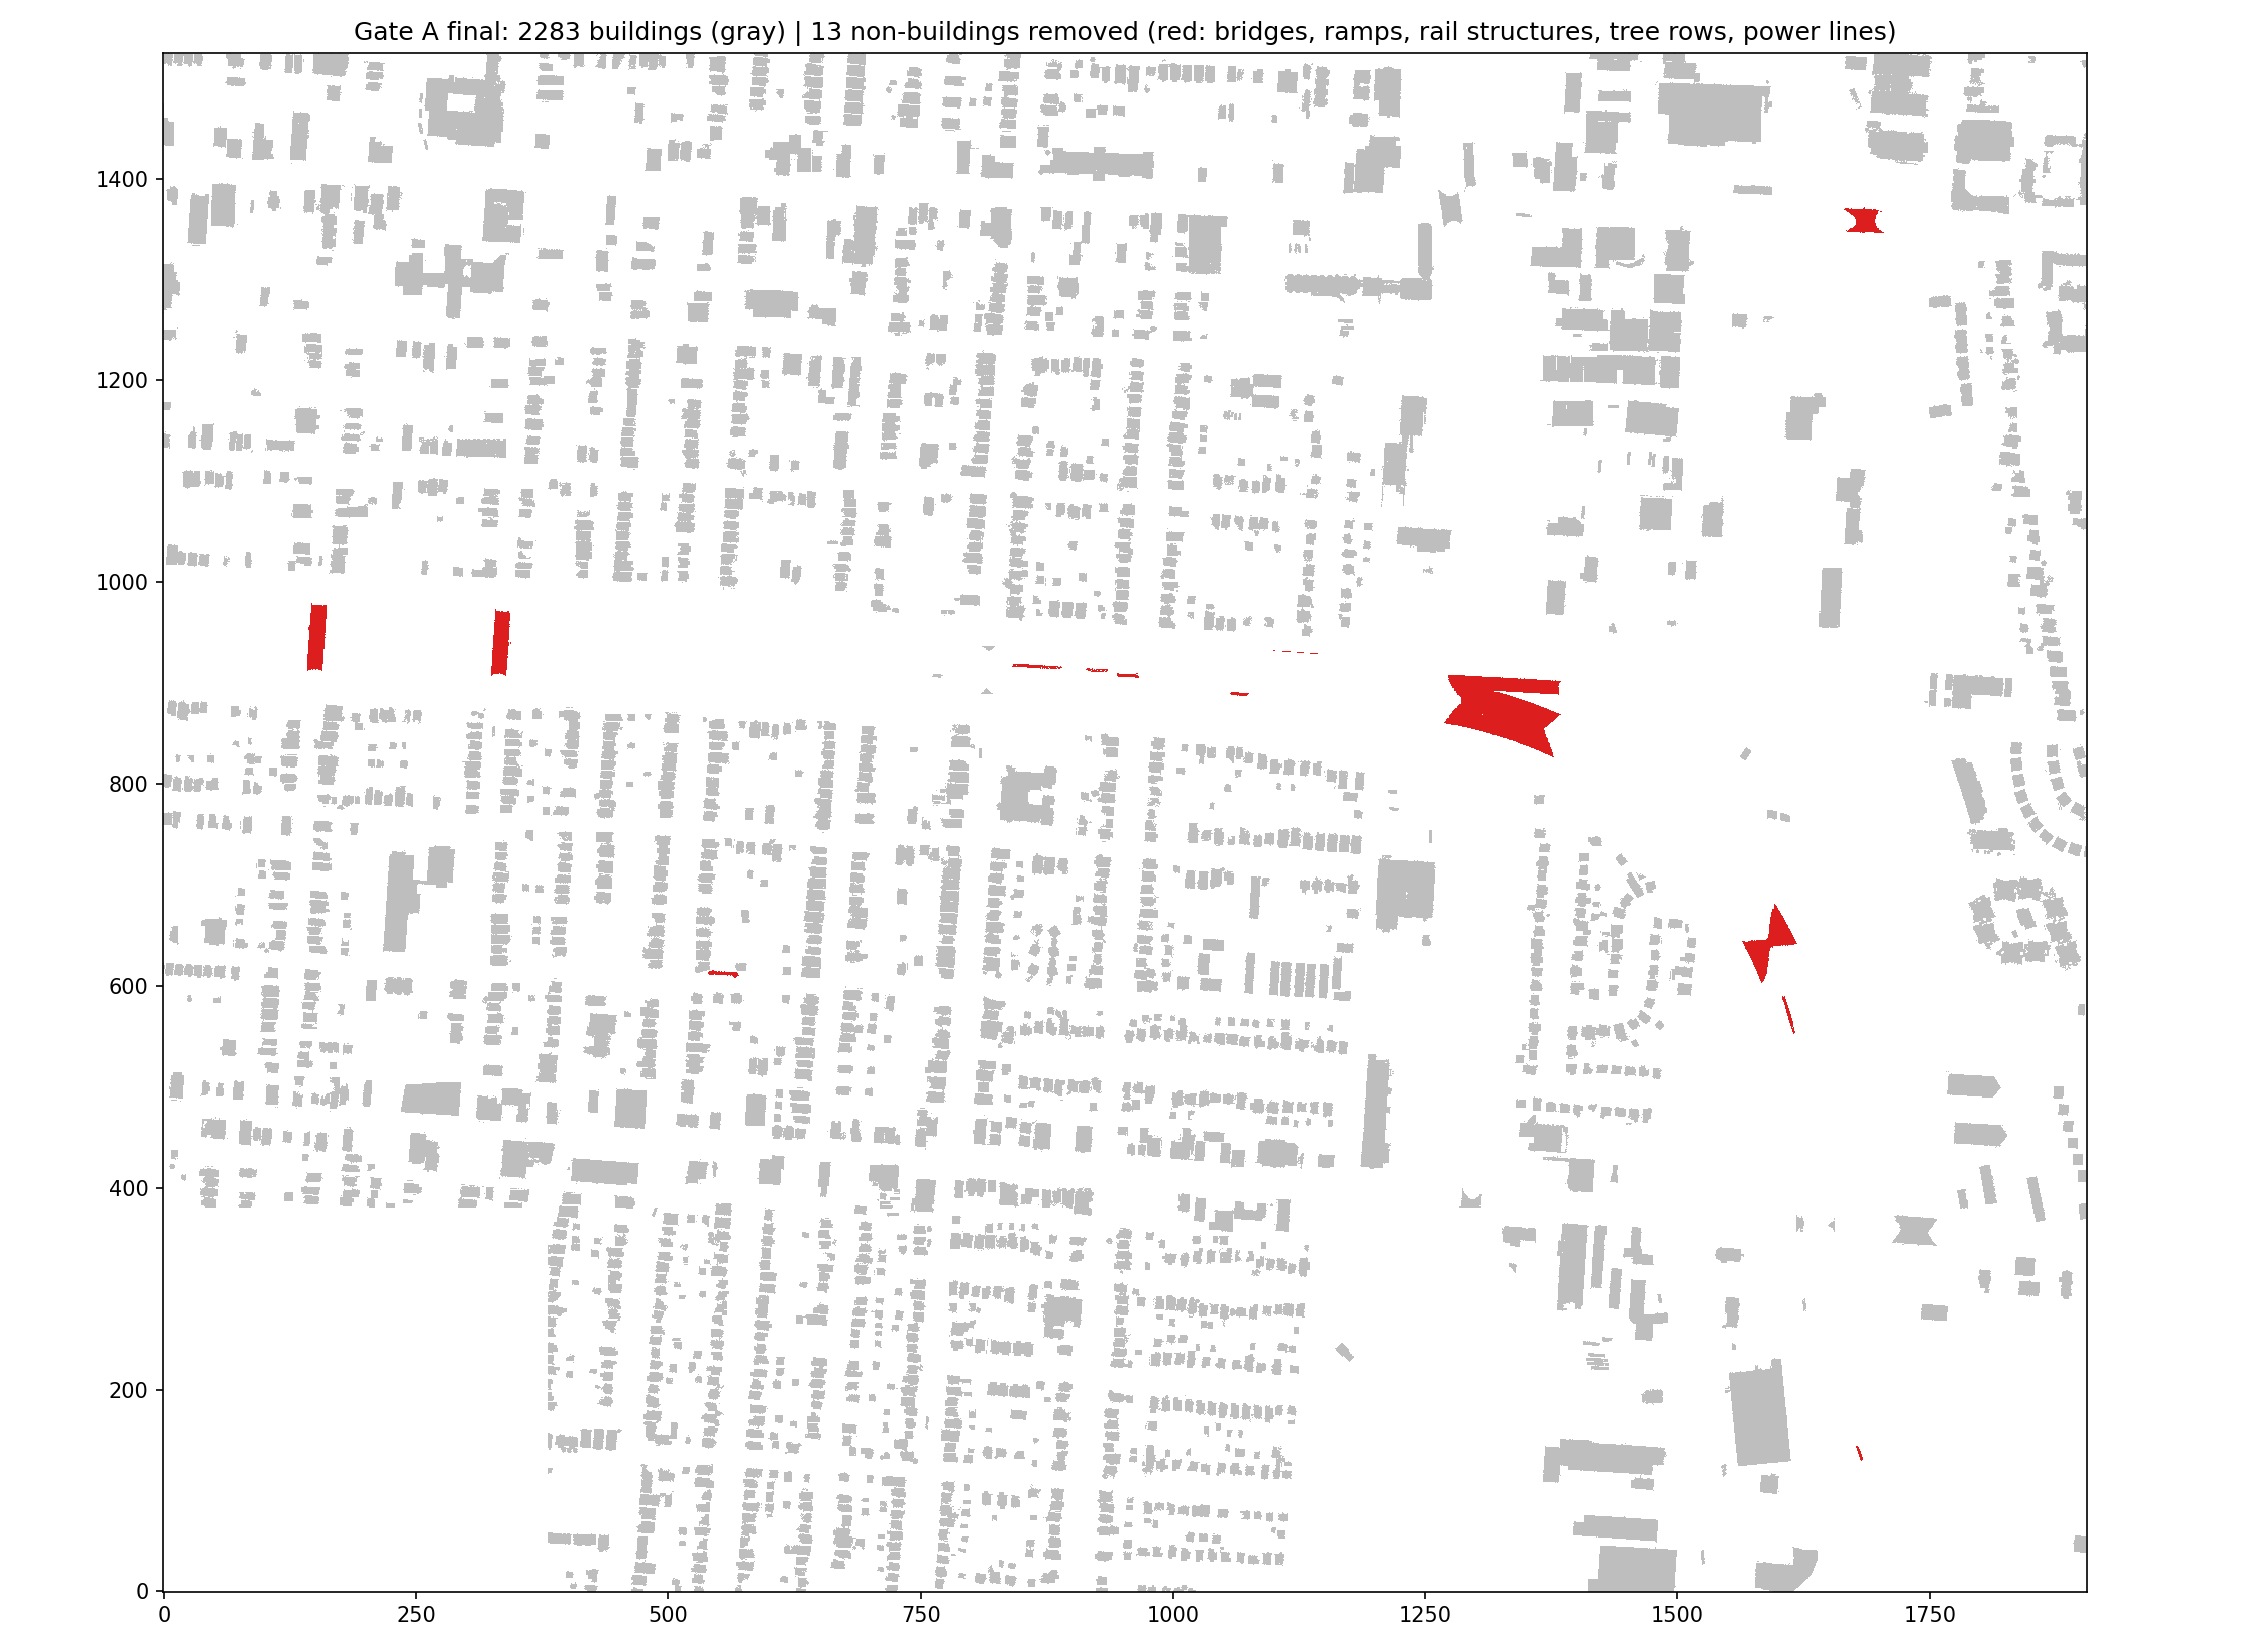
\includegraphics[width=0.95\textwidth]{figs/qa_gateA.png}
\caption{Gate A 审计总图：灰色 = 保留建筑；红色 = 剔除的非建筑。
红色斑块呈带状排列——经与道路/铁路位置核对，剔除对象集中在高速公路与铁路走廊沿线
（图中未叠加路网；做 PPT 时可补一层路网底图佐证）。}
\label{fig:gateA}
\end{figure}

\begin{plainbox}[：模块 5 小结]
\begin{itemize}
\item 假建筑在重建阶段不会自我暴露（桥比楼还平），必须在重建前用实例级特征清除。
\item 三层特征：离地高度 HAG（DTM + 4 m 环 $P_5$，3D BAG 约定）、
      细长度 AR、抗折叠判定量（solidity + elong）。
\item 规则只捞候选、人工定罪、原因码 + 移仓存档全程可审计：
      $2{,}296 \to 2{,}283$。但故事没完——还有两类更隐蔽的错误
      要靠\textbf{后续步骤反馈回来}才能发现，这就是模块 6。
\end{itemize}
\end{plainbox}
